% Standalone: the five population dynamics, redrawn in the panel style
% (cf. rsc/traitors/tex/panel_diagram.tex). This is a restyling of the
% current Table 1 (which should be a figure). Not \input by main.tex.
% Build: pdflatex main.tex
\documentclass[border=4pt]{standalone}
\usepackage{tikz}
\usepackage{amsmath}
\usetikzlibrary{arrows.meta, calc, positioning, shapes.geometric, shapes.symbols}

\definecolor{coop}{HTML}{009E73}     % cooperate
\definecolor{defect}{HTML}{D55E00}   % defect
\definecolor{neutral}{HTML}{8C8C8C}
\definecolor{accent}{HTML}{0072B2}   % selection / extrinsic
\definecolor{warn}{HTML}{E69F00}     % focal marker

\begin{document}
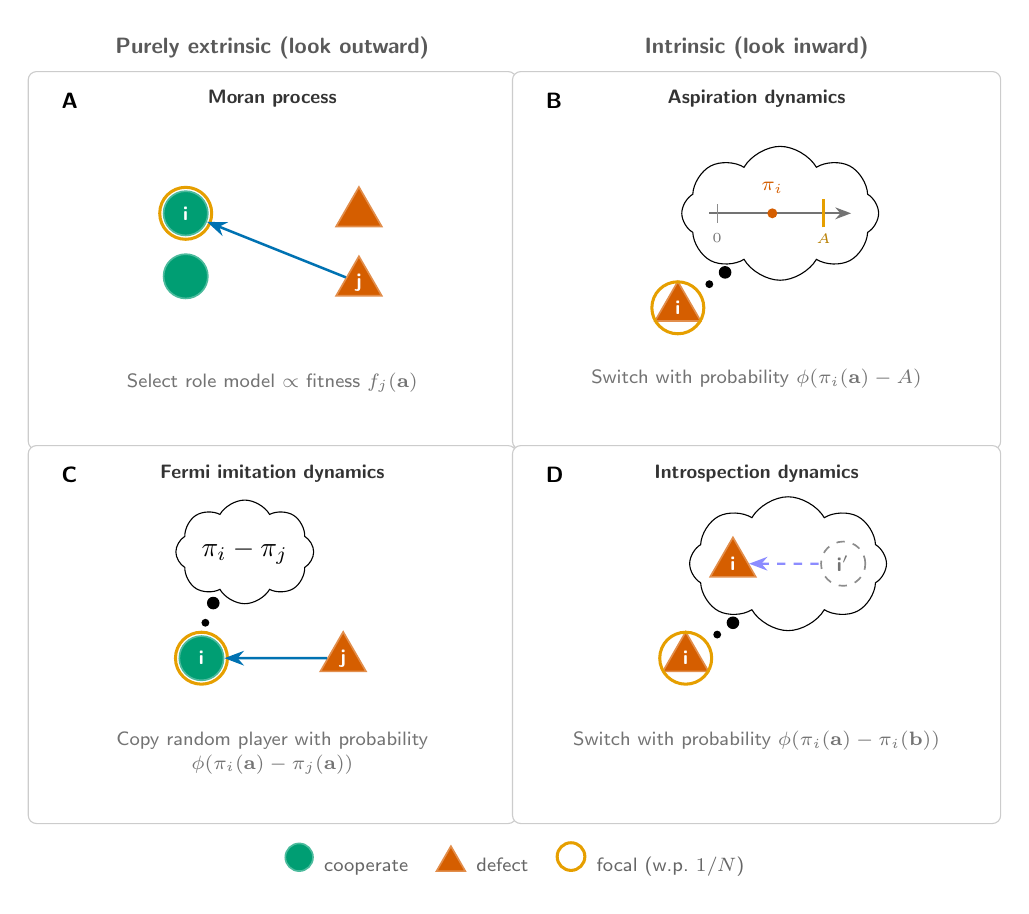
\begin{tikzpicture}[
    >=Stealth,
    font=\sffamily,
    pl/.style={circle, minimum size=16pt, inner sep=0pt, line width=0.6pt,
               font=\sffamily\scriptsize\bfseries, text=white},
    cnode/.style={pl, fill=coop, draw=coop!70},
    dnode/.style={regular polygon, regular polygon sides=3, minimum size=19pt,
                  inner sep=0pt, line width=0.6pt,
                  font=\sffamily\scriptsize\bfseries, text=white,
                  fill=defect, draw=defect!70},
    ghost/.style={circle, minimum size=16pt, inner sep=0pt, line width=0.6pt,
                  font=\sffamily\scriptsize\bfseries, text=black!55,
                  draw=black!45, dashed, fill=white},
    focal/.style={draw=warn, line width=1.1pt},
    panellabel/.style={font=\sffamily\footnotesize\bfseries, anchor=north west},
    ptitle/.style={font=\sffamily\scriptsize\bfseries, text=black!80, align=center},
    note/.style={font=\sffamily\scriptsize, text=black!55, align=center},
    grouphdr/.style={font=\sffamily\footnotesize\bfseries, text=black!65},
    stephdr/.style={font=\sffamily\scriptsize\itshape, text=accent!80!black},
]

\def\pw{5.6}
\def\ph{4.2}
\def\gap{0.55}
\pgfmathsetmacro{\rowtop}{2*\ph+2*\gap}
\pgfmathsetmacro{\rowmid}{\ph+\gap}
\pgfmathsetmacro{\xr}{\pw+\gap}
\pgfmathsetmacro{\wwide}{2*\pw+\gap}

\coordinate (TL) at (0, \rowtop);
\coordinate (TR) at (\xr, \rowtop);
\coordinate (ML) at (0, \rowmid);
\coordinate (MR) at (\xr, \rowmid);
\coordinate (BW) at (0, 0);

% group headers
\node[grouphdr] at (\pw/2, \rowtop+\ph+0.6) {Purely extrinsic (look outward)};
\node[grouphdr] at (\xr+\pw/2, \rowtop+\ph+0.6) {Intrinsic (look inward)};

% A  Moran process (extrinsic)
\begin{scope}[shift=(TL)]
    \draw[draw=black!20, fill=white, rounded corners=3pt]
        (-0.3,-0.3) rectangle (\pw+0.3, \ph+0.3);
    \node[panellabel] at (0, \ph+0.15) {A};
    \node[ptitle] at (\pw/2, \ph-0.05) {Moran process};

    \node[cnode] (Ai) at (1.7,2.7) {i};
    \draw[focal] (Ai) circle (0.33);
    \node[dnode] (Al) at (3.9,2.7) {};
    \node[dnode] (Aj) at (3.9,1.82) {j};
    \node[cnode] (Aw) at (1.7,1.9) {};
    \node[note, text=accent!80!black] at (3.9,3.25) {};

    \draw[->, accent, line width=0.9pt, out=-20] (Aj) -- (Ai);

    \node[note] at (\pw/2,0.55)
        {Select role model $\propto$ fitness $f_j(\mathbf{a})$};
\end{scope}

% C  Fermi imitation dynamics (extrinsic)
\begin{scope}[shift=(ML)]
    \draw[draw=black!20, fill=white, rounded corners=3pt]
        (-0.3,-0.3) rectangle (\pw+0.3, \ph+0.3);
    \node[panellabel] at (0, \ph+0.15) {C};
    \node[ptitle] at (\pw/2, \ph-0.05) {Fermi imitation dynamics};

    \node[cnode] (Bi) at (1.9,1.8) {i};
    \draw[focal] (Bi) circle (0.33);
    \node[dnode] (Bj) at (3.7,1.8) {j};
    %\node[note, text=accent!80!black] at (3.7,3.0) {$j$ picked at random};
    \draw[<-, accent, line width=0.9pt] (Bi) -- (Bj);

    % thought bubble
    \node[
        cloud,
        cloud puffs=8,
        cloud puff arc=120,
        aspect=1.6,
        draw,
        fill=white,
        minimum width=0.9cm,
        minimum height=0.45cm,
        inner sep=1pt
    ] (thought) at ($(Bi)+(0.55,1.35)$) {$\pi_i-\pi_j$};

    % connecting bubbles
    \fill ($(Bi)+(0.05,0.45)$) circle (0.05);
    \fill ($(Bi)+(0.15,0.70)$) circle (0.08);

    \node[note] at (\pw/2,0.75)
        {Copy random player with probability};

    \node[note] at (\pw/2,0.45)
        {$\phi\!\left(\pi_i(\mathbf{a})-\pi_j(\mathbf{a})\right)$};
\end{scope}

% B  Aspiration dynamics (intrinsic)
\begin{scope}[shift=(TR)]
    \draw[draw=black!20, fill=white, rounded corners=3pt]
        (-0.3,-0.3) rectangle (\pw+0.3, \ph+0.3);
    \node[panellabel] at (0, \ph+0.15) {B};
    \node[ptitle] at (\pw/2, \ph-0.05) {Aspiration dynamics};

    \node[dnode] (Ci) at (1.8,1.5) {i};
    \draw[focal] (Ci) circle (0.33);

    \node[
        cloud,
        cloud puffs=8,
        cloud puff arc=120,
        aspect=1.6,
        draw,
        fill=white,
        minimum width=2.5cm,
        minimum height=1.7cm,
        inner sep=1pt
    ] (thought) at ($(Ci)+(1.3,1.2)$) {};

    \fill ($(Ci)+(0.4,0.3)$) circle (0.05);
    \fill ($(Ci)+(0.6,0.45)$) circle (0.08);

    \draw[->, black!55, line width=0.6pt]
        ($(thought.center)+(-0.90,0)$) --
        ($(thought.center)+( 0.90,0)$);

    \draw[black!45]
        ($(thought.center)+(-0.80,-0.12)$) --
        ($(thought.center)+(-0.80, 0.12)$);

    \draw[warn, line width=1pt]
        ($(thought.center)+(0.55,-0.18)$) --
        ($(thought.center)+(0.55, 0.18)$);

    \node[font=\sffamily\tiny, text=black!55]
        at ($(thought.center)+(-0.80,-0.32)$) {$0$};

    \node[font=\sffamily\tiny, text=warn!80!black]
        at ($(thought.center)+(0.55,-0.32)$) {$A$};

    \node[font=\sffamily\scriptsize, text=defect]
        at ($(thought.center)+(-0.10,0.32)$) {$\pi_i$};

    \fill[defect]
        ($(thought.center)+(-0.10,0)$) circle (1.8pt);

    \node[note] at (\pw/2,0.6)
        {Switch with probability $\phi\!\left(\pi_i(\mathbf{a})-A\right)$};
\end{scope}

% D  Introspection dynamics (intrinsic)
\begin{scope}[shift=(MR)]
    \draw[draw=black!20, fill=white, rounded corners=3pt]
        (-0.3,-0.3) rectangle (\pw+0.3, \ph+0.3);
    \node[panellabel] at (0, \ph+0.15) {D};
    \node[ptitle] at (\pw/2, \ph-0.05) {Introspection dynamics};

    \node[dnode] (Di) at (1.9,1.8) {i};
    \draw[focal] (Di) circle (0.33);

    \node[
            cloud,
            cloud puffs=8,
            cloud puff arc=120,
            aspect=1.6,
            draw,
            fill=white,
            minimum width=2.5cm,
            minimum height=1.7cm,
            inner sep=1pt
        ] (thought) at ($(Di)+(1.3,1.2)$) {};

    % connecting bubbles
    \fill ($(Di)+(0.4,0.3)$) circle (0.05);
    \fill ($(Di)+(0.6,0.45)$) circle (0.08);

    \node[ghost] (ghost) at ($(thought.center) + (0.7, 0)$) {i$'$};
    \node[dnode] (Di_thought) at ($(thought.center) - (0.7, 0)$) {i};
    \draw[<-, blue!45, line width=0.8pt, dashed] (Di_thought) -- (ghost);
    %\node[note] at (3.7,2.72) {counterfactual};
    %\node[note, text=accent!80!black] at (1.9,3.15) {action picked at random};

    \node[note] at (\pw/2,0.75)
        {Switch with probability $\phi\!\left(\pi_i(\mathbf{a})-\pi_{i}(\mathbf{b})\right)$};
\end{scope}

% legend
\node[font=\sffamily\scriptsize, text=black!60] at (\wwide/2,\rowmid-0.75)
    {\tikz\node[cnode, minimum size=10pt]{};\, cooperate \quad
     \tikz\node[dnode, minimum size=12pt]{};\, defect \quad
     \tikz\draw[focal] (0,0) circle (5pt);\, focal (w.p.\ $1/N$)};

\end{tikzpicture}
\end{document}
